% The article body
% Also see main.tex for information such as authors, title, etc
% See https://www.overleaf.com/learn/ for some great resources on learning latex

\section{Introdução}
Resolução da lista de exercício, da aula do dia 28 de fevereiro de 2023.

\section{Questionário}

\subsection{Qual a faixa de condutividade para materiais isolantes, semicondutores e condutores?}
Em $\left[\Omega^{-1}\cdot m^{-1}\right]$:\\
Isolantes: de $10^{-8}$ à $10^{-18}$\\
Semicondutores: de $10^{2}$ à $10^{4}$\\
Condutores: de $10^{4}$ à $10^{8}$
\subsection{Qual a importância de se estudar as ligações químicas para o estudo de dispositivos elétricos?}
O estudo das ligações químicas é muito importante pois eletricidade é a transferência de elétrons entre átomos, sendo assim determinando níveis de condutividade, e outras caracteríticas para o semicondutor.
\subsection{Explique como se formam os 3 tipos de ligações primárias.}
Ligação iônica: Ocorre entre átomos de elementos diferentes que possuem uma grande diferença de eletronegatividade, ou seja, a capacidade de atrair elétrons. Nessa ligação, os átomos perdem ou ganham elétrons para formar íons com cargas opostas, que se atraem e formam um composto iônico.\\
Ligação covalente: Ocorre quando dois átomos compartilham elétrons para formar uma molécula. Essa ligação ocorre entre átomos com eletronegatividades semelhantes e pode ser polar ou apolar, dependendo da distribuição dos elétrons.\\
Ligação metálica: Ocorre entre átomos de metais e é caracterizada pela formação de uma rede cristalina tridimensional, na qual os elétrons dos átomos de metal são compartilhados por todos os átomos da rede. Isso dá origem a um arranjo de átomos que é altamente condutor de eletricidade e calor.
\subsection{Por que a indústria microeletrônica está baseada em Si?}
A indústria microeletrônica está baseada no silício (Si) devido às suas propriedades únicas e favoráveis para a fabricação de dispositivos eletrônicos.
O silício é o segundo elemento mais abundante na crosta terrestre, o que significa que ele é relativamente barato e fácil de obter em grandes quantidades. O silício é também um elemento muito estável, o que facilita o seu processamento e fabricação em larga escala. Outro fator importante é que o silício é um elemento tetravalente, o que significa que cada átomo de silício pode formar quatro ligações covalentes com outros átomos de silício. Essa propriedade permite a criação de uma rede cristalina tridimensional, que é a base para a fabricação de dispositivos microeletrônicos.
\subsection{Por que os metais apresentam alta condutividade elétrica e térmica e alta opacidade?}
Os metais apresentam alta condutividade elétrica e térmica devido à sua estrutura atômica particular. Os átomos de metal são organizados em um arranjo cristalino que permite que os elétrons de valência se movam facilmente através da estrutura, criando uma rede tridimensional de elétrons que é compartilhada por todos os átomos na rede.
Quando uma tensão elétrica é aplicada aos metais, os elétrons de valência são liberados e começam a se mover através da rede de átomos. Esses elétrons se movem rapidamente de átomo para átomo, transportando a carga elétrica através do material. O mesmo princípio se aplica à condutividade térmica, pois o movimento dos elétrons de valência também transporta a energia térmica através do material.

A alta opacidade dos metais se deve à sua capacidade de absorver e refletir a luz. Quando a luz atinge a superfície do metal, os elétrons na nuvem de elétrons absorvem a energia da luz e começam a oscilar. Essa oscilação absorve a energia da luz e não permite que ela passe através do metal, tornando o metal opaco à luz visível.
\subsection{Explique sucintamente as etapas de obtenção de um silício de grau metalúrgico.}
As etapas para obtenção de silício de grau metalúrgico envolvem mineração, purificação, redução e refino, utilizando técnicas químicas e físicas para produzir um silício metálico puro e com as características desejadas
\subsection{Explique sucintamente as etapas de obtenção do Si policristalino grau eletrônico.}
As etapas para obtenção de silício policristalino grau eletrônico envolvem redução, purificação, fundição, corte e polimento, utilizando técnicas químicas e físicas para produzir wafers de silício policristalino com as características desejadas para a fabricação de dispositivos eletrônicos
\subsection{Explique sucintamente a formação do monocristal de Si pelo método de FZ (floating zone) e Cz (Czochralski).}
A formação de monocristais de silício pode ser realizada pelo método de FZ (Floating Zone) ou pelo método de Cz (Czochralski). Ambos os métodos envolvem a fusão do silício em um forno de alta temperatura e a solidificação controlada para formar um monocristal. As principais diferenças entre os dois métodos são:

Método de FZ: envolve a fusão de um pequeno pedaço de silício em um forno de alta frequência, gerando uma zona de fusão que é movida lentamente através do lingote. Durante a solidificação, um único cristal é formado na região onde a zona de fusão encontra a porção sólida do lingote. Este método é utilizado para produzir monocristais de alta qualidade com baixas concentrações de impurezas.

Método de Czochralski (Cz): envolve a fusão de silício em um cadinho e, em seguida, a inserção de um cristal semente que inicia o crescimento do monocristal. Durante o processo de crescimento, o cristal é lentamente puxado para cima enquanto a temperatura é controlada para produzir um monocristal de silício cilíndrico. Este método é mais utilizado em escala industrial e é capaz de produzir grandes volumes de monocristais de silício, mas pode apresentar maiores concentrações de impurezas em comparação ao método de FZ.
\subsection{Por que se realizam chanfros no Si monocristalino?}
Os chanfros são realizados no Si monocristalino durante o processo de fabricação dos wafers, para evitar rachaduras nas bordas do cristal durante a manipulação e a montagem. Além disso, os chanfros são úteis para evitar que as bordas do cristal danifiquem o equipamento ou as ferramentas utilizadas no processo de fabricação.
Os chanfros também podem ser usados para distinguir a orientação cristalina do Si monocristalino, já que os ângulos de chanfro são definidos em relação às diferentes orientações cristalinas do material.

\subsection{Explique o funcionamento de um diodo em termos de difusão de portadores, região de 
depleção e barreira de potencial. Explique o diodo na polarização direta e reversa.}
Um diodo é um dispositivo eletrônico composto por uma junção PN formada pela união de um material semicondutor tipo P e um material semicondutor tipo N. O funcionamento do diodo está relacionado com a difusão de portadores de carga através da junção PN e a formação de uma região de depleção.

Na região de depleção, os portadores de carga livre (elétrons no material tipo N e lacunas no material tipo P) se recombinam, deixando a região com uma concentração muito baixa de portadores. Isso gera uma carga elétrica positiva na região N adjacente à junção e uma carga negativa na região P adjacente à junção, criando um campo elétrico interno que impede a difusão adicional de portadores através da junção.

Quando o diodo é polarizado diretamente, a tensão aplicada no dispositivo faz com que o potencial elétrico da região P fique maior que o da região N, diminuindo a barreira de potencial na junção PN e permitindo que os portadores de carga se difundam através da junção. Isso resulta em uma corrente elétrica que flui através do diodo. Nessa polarização, a região de depleção diminui, e o diodo passa a ter uma resistência elétrica baixa, permitindo a passagem de corrente elétrica.

Já na polarização reversa, a tensão aplicada no dispositivo faz com que o potencial elétrico da região N fique maior que o da região P, aumentando a barreira de potencial na junção PN e ampliando a região de depleção. Isso impede que os portadores de carga se difundam através da junção, tornando a resistência elétrica do diodo muito alta, praticamente impedindo a passagem de corrente elétrica.
\subsection{Explique o funcionamento do transistor bipolar no modo ativo.}
O funcionamento do transistor bipolar no modo ativo está relacionado com a injeção de portadores de carga do emissor para a base, gerando um excesso de portadores majoritários na região da base e permitindo a difusão de portadores do excesso de portadores da base para o coletor, o que gera uma corrente de elétrons no coletor, que é controlada pela corrente de base. O transistor bipolar no modo ativo é utilizado em amplificadores de corrente e em diversos outros dispositivos eletrônicos.
\subsection{Dadas as curvas características de entrada (a) e saída (b) de um transistor NPN, determinar:}

\begin{figure}[h!]
\subfloat[Entrada]{
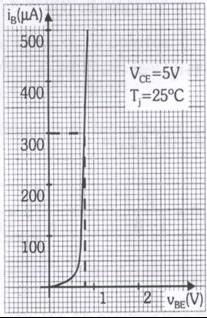
\includegraphics[height=0.28\textheight]{entrada.png}}
\hspace*{\fill}
\subfloat[Saída]{%
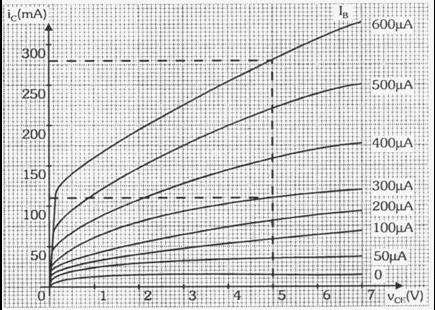
\includegraphics[height=0.28\textheight]{saida.png}}
\caption{Curvas características de um transistor NPN}
\end{figure}

\noindent a) A corrente de base para $V_{BE} = 0,8 V$;
\begin{equation} i_B = 300 \mu A \label{eq0}\end{equation}
\noindent b) O ganho de corrente nas condições do item a);
\begin{equation} \beta = \frac{i_C}{i_B}  = \frac{110 mA}{300 \mu A} \label{eq1}\end{equation}
\begin{equation} \beta = 366,67 \label{eq2}\end{equation}

\noindent c) O novo ganho de corrente, caso IB dobre de valor, mantida a tensão $V_{CE}$.
\begin{equation} \beta_2 = \frac{i_{C2}}{i_{B2}}  = \frac{280 mA}{600 \mu A} \label{eq3}\end{equation}
\begin{equation} \beta_2 = 466,67 \label{eq4}\end{equation}
  

